
\documentclass{beamer}
\usetheme{Electromagnetism}
\usepackage{Electromagnetism}
\graphicspath{{pictures/}}
\usepackage{cancel}
% -------------------------------------- Grid
%-------------------------------------------------------
\makeatletter
\def\grd@save@target#1{%
  \def\grd@target{#1}}
\def\grd@save@start#1{%
  \def\grd@start{#1}}
\tikzset{
  grid with coordinates/.style={
    to path={%
      \pgfextra{%
        \edef\grd@@target{(\tikztotarget)}%
        \tikz@scan@one@point\grd@save@target\grd@@target\relax
        \edef\grd@@start{(\tikztostart)}%
        \tikz@scan@one@point\grd@save@start\grd@@start\relax
        \draw[minor help lines, gray!50] (\tikztostart) grid (\tikztotarget);
        \draw[major help lines, gray!50] (\tikztostart) grid (\tikztotarget);
        \grd@start
        \pgfmathsetmacro{\grd@xa}{\the\pgf@x/1cm}
        \pgfmathsetmacro{\grd@ya}{\the\pgf@y/1cm}
        \grd@target
        \pgfmathsetmacro{\grd@xb}{\the\pgf@x/1cm}
        \pgfmathsetmacro{\grd@yb}{\the\pgf@y/1cm}
        \pgfmathsetmacro{\grd@xc}{\grd@xa + \pgfkeysvalueof{/tikz/grid with coordinates/major step}}
        \pgfmathsetmacro{\grd@yc}{\grd@ya + \pgfkeysvalueof{/tikz/grid with coordinates/major step}}
        \foreach \x in {\grd@xa,\grd@xc,...,\grd@xb}
        \node[anchor=north] at (\x,\grd@ya) {\pgfmathprintnumber{\x}};
        \foreach \y in {\grd@ya,\grd@yc,...,\grd@yb}
        \node[anchor=east] at (\grd@xa,\y) {\pgfmathprintnumber{\y}};
      }
    }
  },
  minor help lines/.style={
    help lines,
    step=\pgfkeysvalueof{/tikz/grid with coordinates/minor step}
  },
  major help lines/.style={
    help lines,
    line width= 0.5pt,
    step=\pgfkeysvalueof{/tikz/grid with coordinates/major step}
  },
  grid with coordinates/.cd,
  minor step/.initial=.2,
  major step/.initial=1,
  major line width/.initial=2pt,
}
\makeatother

\begin{document}

% ============================== Слайд ## ===================================
\begin{frame}{Вектор-потенціал на далеких відстанях}{}
	\begin{columns}
		\begin{column}{0.3\linewidth}
			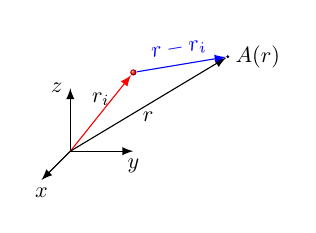
\begin{tikzpicture}[>=latex, scale=0.8, transform shape]
				\draw[->] (0,0) -- ++(1, 0) node[below] {$y$};
				\draw[->] (0,0) -- ++(0, 1) node[left] {$z$};
				\draw[->] (0,0) -- ++({180+45}:0.65) node[below] {$x$};

				\node[circle, inner sep=1pt, ball color=red] (i1) at (1, 1.25) {};
				\node[circle, inner sep=0.5, fill] (P) at (2.5, 1.5) {};
				\node[right] at (P) {$\vect{A}(\vect{r})$};

				\draw[->, red] (0,0) -- node[above, text=black] {$\vect{r}_i$} (i1);
				\draw[->] (0,0) -- node[below] {$\vect{r}$} (P);
				\draw[->, blue] (i1) -- node[above, sloped] {$\vect{r} - \vect{r}_i$} (P);
			\end{tikzpicture}
		\end{column}
		\begin{column}{0.7\linewidth}
			Магнітний момент системи тіл:
			\begin{equation*}
				\vect{A} = \frac1c \sum_i \frac{q_i\vect{v_i}}{|\vect{r} - \vect{r}_i|}
			\end{equation*}
		\end{column}
	\end{columns}
	\begin{overprint}
		\onslide<1>
		\begin{block}{}
			На далеких відстанях $r_i \ll r$ наближено
			\(
			\frac{1}{|\vect{r} - \vect{r}_i|} \approx \frac1r \left(1 + \frac{\vect{r}\ \vect{r}_i}{r^2}\right).
			\)
		\end{block}
		\begin{alertblock}{}\justifying\small
			Для стаціонарних рухів, які відбуваються в малих областях, можна зробити усереднення вектор-потенціалу, при цьому
			$\overline{\frac{d}{dt}\ldots}
				=
				0$.
		\end{alertblock}
		\begin{equation*}
			\overline{\vect{A}} = \frac1{cr^3} \sum_iq_i\overline{v_i(\vect{r}\ \vect{r}_i)}
		\end{equation*}
		\begin{center}\footnotesize
			\begin{equation*}
				v_i(\vect{r}\ \vect{r}_i) = \frac12\left[v_i(\vect{r}\ \vect{r}_i) - \vect{r}_i(\vect{r}\ \vect{v}_i)\right] + \frac12\left[v_i(\vect{r}\
					\vect{r}_i) + \vect{r}_i(\vect{r}\ \vect{v}_i)\right]
				= \frac12 \vect{r}\times\vect{v}_i\times\vect{r}_i + \frac12\frac{d}{dt}\left(\vect{r}_i(\vect{r}\ \vect{r}_i)\right).
			\end{equation*}
		\end{center}
		\onslide<2>
		\begin{equation*}
			\overline{\vect{A}} =  \frac1{r^3}  \left(\frac1{2c} \sum_i \vect{r}_i\times (q_i\vect{v}_i)\right)\times\vect{r} =
			\frac{\vect{p}_m\times\vect{r}}{r^3} .
		\end{equation*}
		Магнітне поле знаходиться за формулою $\Bfield = \Rot\vect{A}$:
		{\scriptsize%
		\begin{align*}
			\Rot\vecdot{\vect{A}}{\vect{B}}                                 & = \scdot{\vect{B}}{\grad}\vect{A} - \scdot{\vect{A}}{\grad}\vect{B} + 	\vect{A}\Div\vect{B} -
			\vect{B}\Div\vect{A}                                                                                                                                            \\
			\Bfield = \Rot\left(\vect{p}_m\times\frac{\vect{r}}{r^3}\right) & =                                                                                             %\cancelto{0}{\vect{p}_m\Div\frac{\vect{r}}{r^3}}
			-\scdot{\vect{p}_m}{\grad}\frac{\vect{r}}{r^3} = \frac{3\scdot{\vect{p}_m}{\vect{r}}\vect{r}}{r^5} - \frac{\vect{p}_m}{r^3}.
		\end{align*}
		}
		\begin{equation*}
			\Bfield = \frac{3\scdot{\vect{p}_m}{\vect{r}}\vect{r}}{r^5} - \frac{\vect{p}_m}{r^3}.
		\end{equation*}
	\end{overprint}
\end{frame}
% ===========================================================================

% ============================== Слайд ## ===================================
\begin{frame}{Магнітний диполь}{}
	\begin{block}{}
		\begin{columns}
			\begin{column}{0.7\linewidth}
				\begin{block}{}\justifying
					\begin{equation*}
						\tcbhighmath{\Bfield = \frac{3\scdot{\vect{p}_m}{\vect{r}}\vect{r}}{r^5} - \frac{\vect{p}_m}{r^3}.}
					\end{equation*}
					{\scriptsize Отримана формула збігається за виглядом із формулою для електричного поля точкового диполя. Це означає, що точковий
					магнітний момент можна розглядати формально як точковий диполь, складений з ефективних магнітних зарядів\\ \textcolor{red}{$N$}
					(\textcolor{red}{північного}) та \textcolor{blue}{$S$} (\textcolor{blue}{південного}).}
				\end{block}
			\end{column}
			\begin{column}{0.3\linewidth}
				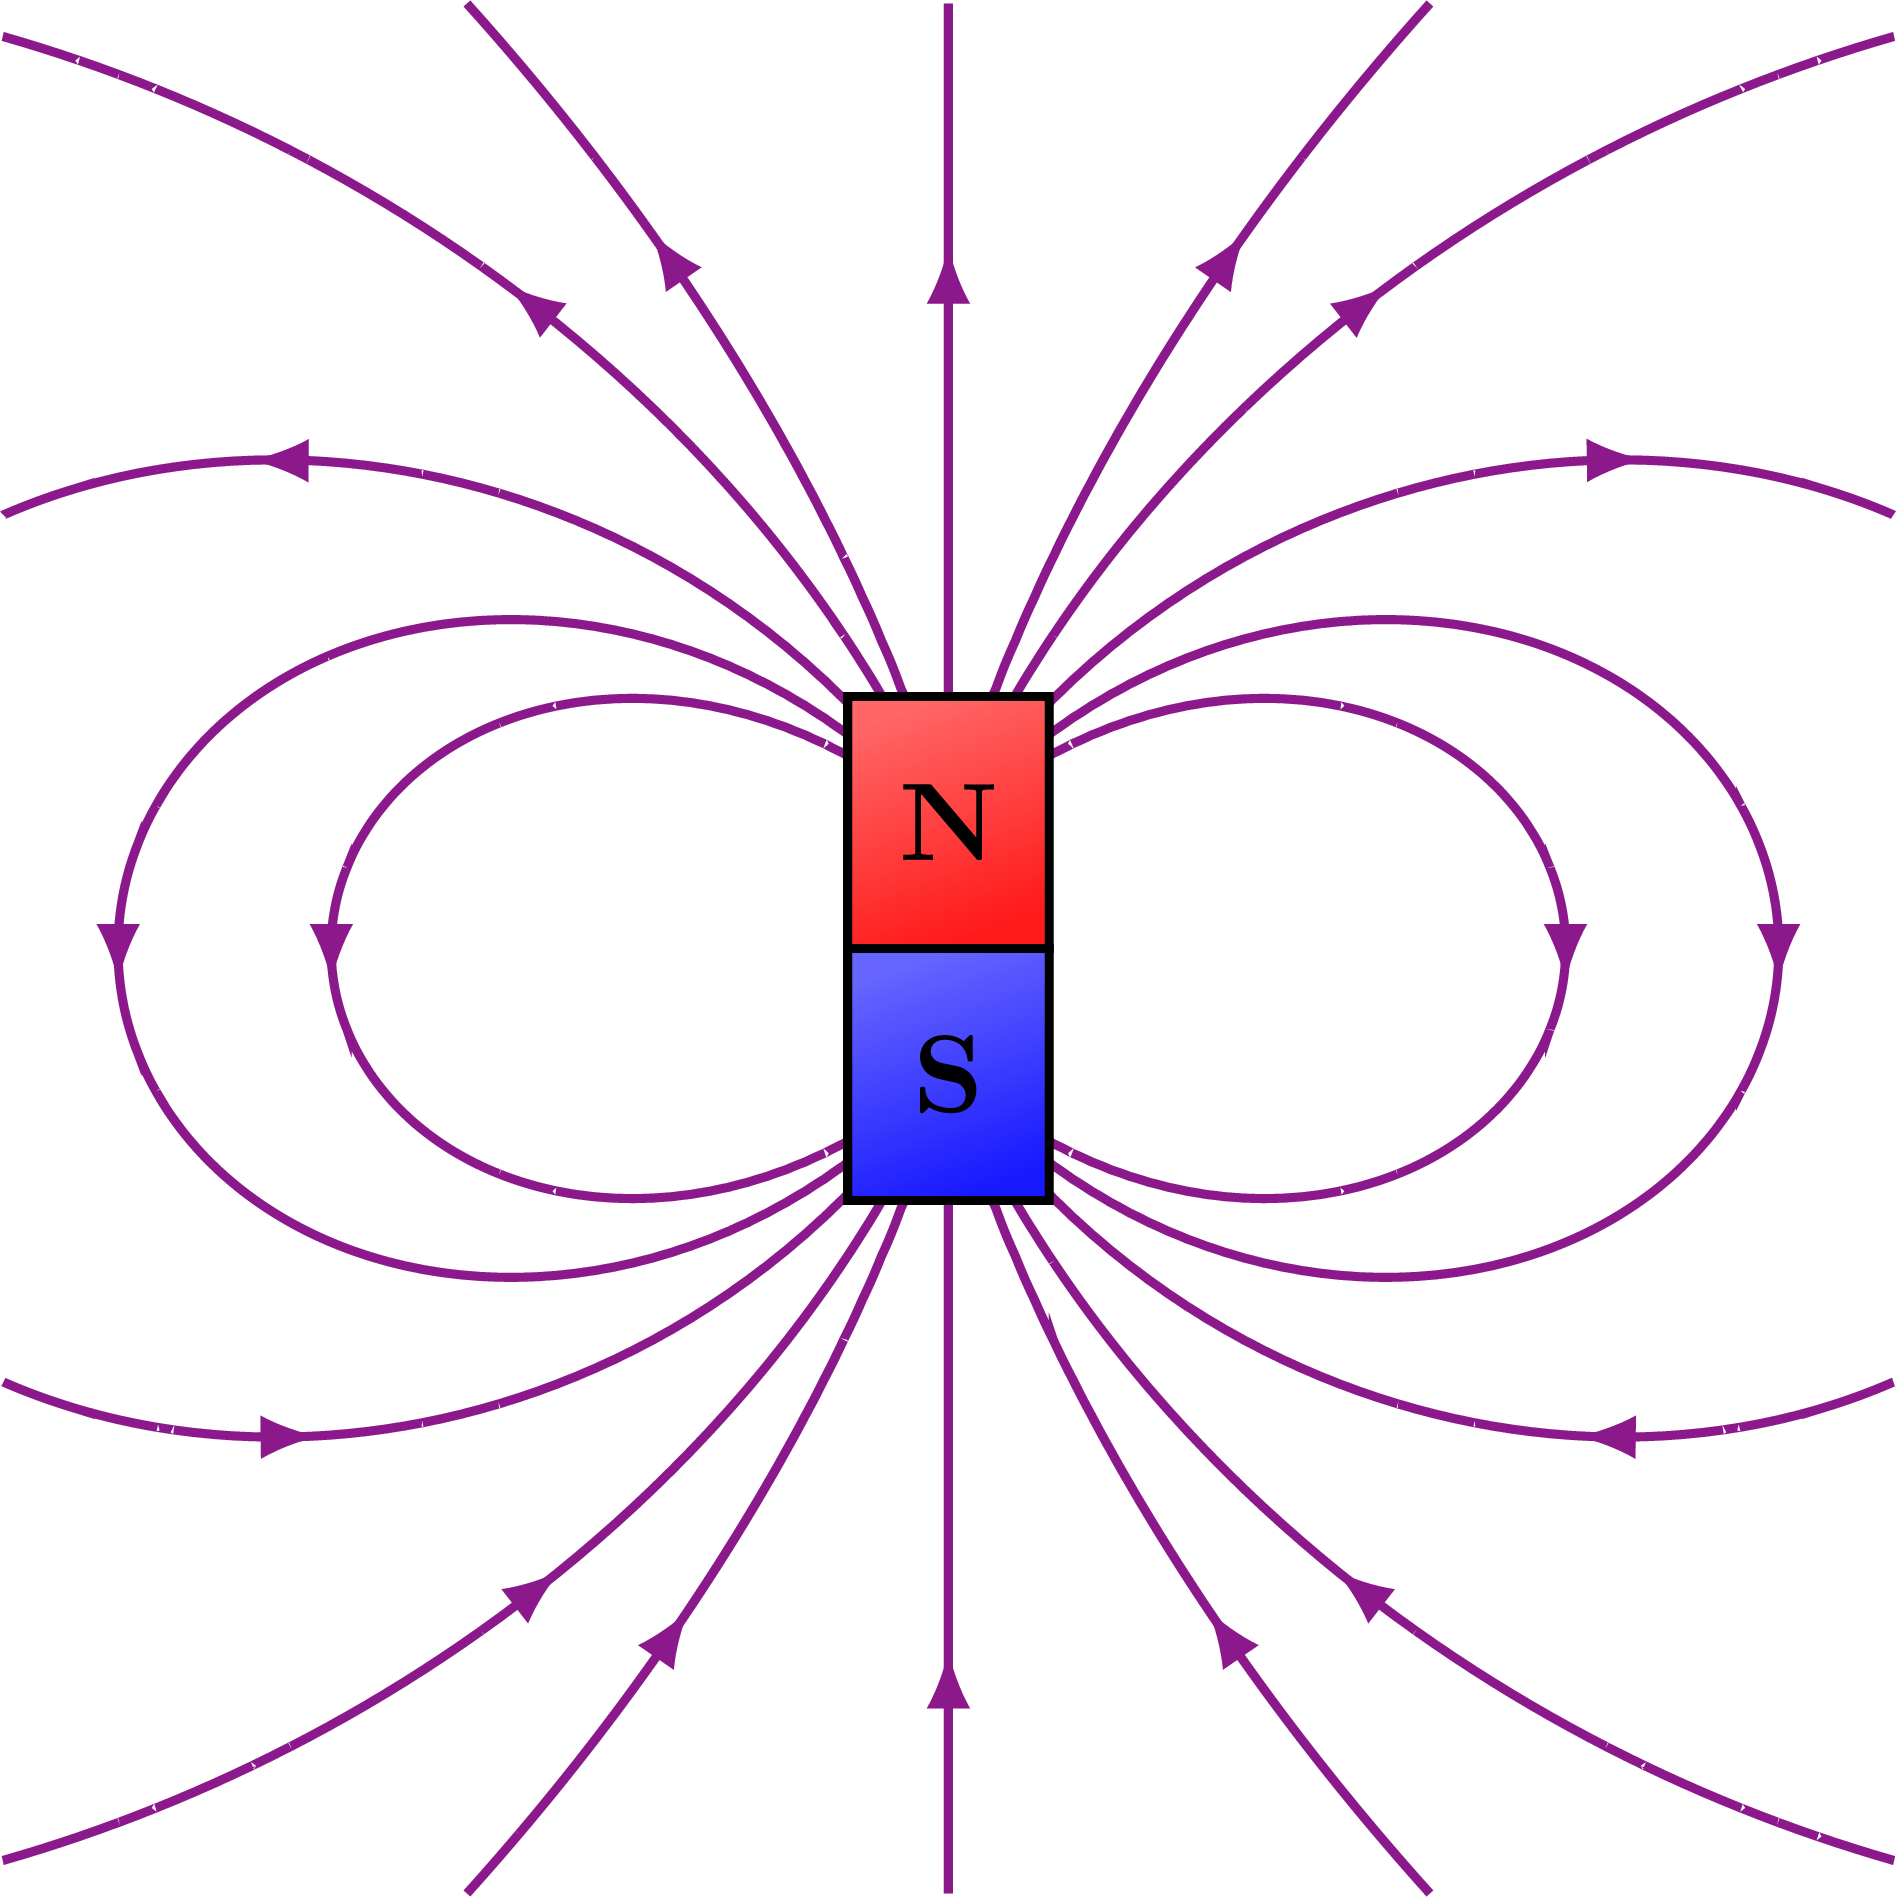
\includegraphics[width=\linewidth]{magdipole}
			\end{column}
		\end{columns}

	\end{block}
	\begin{center}\small
		\begin{tblr}%
			{
			colspec={Q[l,m]X[c,m]X[c,m]},
            cell{1}{2,3} = {fg=white, bg=cyan},
            cell{2,3}{1} = {fg=white, bg=cyan},
			hlines,
			vlines,
			}
			          & Електричний диполь                                                                      & Магнітний диполь                                  \\
			%			Означення & $\vect{p}_e = \iiint\limits_V \rho dV$                                                  & $\vect{p}_m = \frac1{2c}
			%\iiint\limits_V \vect{r}\times \rho\vect{v}\ dV$ \\
			Потенціал & $\phi = \dfrac{\vect{p}_e\cdot\vect{r}}{r^3}$                                            & $\vect{A} =
			\dfrac{\vect{p}_m\times\vect{r}}{r^3}$ \\
			Поле      & $\Efield = \dfrac{3\scdot{\vect{p}_e}{\vect{r}}\vect{r}}{r^5} - \dfrac{\vect{p}_e}{r^3} $ & $\Bfield =
			\dfrac{3\scdot{\vect{p}_m}{\vect{r}}\vect{r}}{r^5} -
			\dfrac{\vect{p}_m}{r^3}$                                                                             \\
		\end{tblr}
	\end{center}
\end{frame}
% ===========================================================================


\end{document}